
\section{Results}
\label{mmf-sec:results}
In this section I will present the results when applying MisMatchFinder to various different datasets. First the evaluation of the method on simulated data, which allows accurate and definitive insight into the sensitivity and a proof of concept (\autoref{mmf-sec:simulated data}). Then the analysis of real world applications is displayed in \autoref{mmf-sec:realworld} demonstrating that the method does not only work in cleanly simulated data, but find clinically relevant insight in patient samples.

\subsection{Simulated Data - the validation promised land}
\label{mmf-sec:simulated data}
Just like in \autoref{ch:variantcalling}, the novelty of the approach leads to the issue of no gold standard dataset, with which to evaluate the performance of a new method. While there are low coverage WGS datasets of cancer patients, none of them have validated signatures associated with them. So again simulated data is the optimal starting point to allow both optimisation of parameters as well as granular detection of artefacts which can originate from any step starting from sequencing over mapping to the signature deconvolution. 

\subsubsection{Sequencing errors - there is always a cleaner data}
\label{mmf-sec:cleanSim}
To judge the ability of our approach to filter out sequencing errors, we first simulated ``clean`` sequencing reads with neither germline or somatic variants with the ART simulation suite \cite{Huang2011}. As current estimates of Illumina sequencing is in the range of 1 in 666 to 1 in 1149 \cite{Stoler2021} which is significantly higher than even the highest tumour mutational burdens of  cancers (melanoma: 1 in 5k; tobacco smoking lung cancer: 1 in 100k) it is very important to be able to eliminate as much of the  background noise of sequencing errors as possible.

\begin{figure}[!ht]
\centering
\includegraphics[width=.99\linewidth]{Figures/mismatchrateCleanSequencing.pdf}
\caption[Mismatchrate of different filtering methods]{Mismatchrate of different filtering methods on sequencing data simulated with ART\cite{Huang2011} for both 10x and 3x coverage; Mismatches correspond to simulated sequencing errors; all: no filters, overlap: only use the overlapping parts of paired end reads with consensus building (\protect\autoref{mmf-sec:consensus}), strict OL: overlap but reads \emph{must} agree, high BQ strict OL: strict OL with high BQ in both variants; A) Absolute counts B) counts from A normalised by the number of analysed bases all: all aligned bases, other: number of bases in read overlap}\label{fig:mmf-mismatchrate}
\end{figure}

By only using high base quality mismatches, where both reads agree on the mismatch 99.98\% of all sequencing errors can be eliminated and only 1 in 10M bases will be wrongly counted as a variant (\autoref{fig:mmf-mismatchrate}). This false discovery rate is multiple orders of magnitude lower than before and in a similar range to normal mutationally driven cancers tumour mutational burden \cite{Alexandrov2020,Lawrence2013a}.


\subsubsection{Spike-in signature detection}
\label{mmf-sec:simSingnatures}
With the technical error eliminated in simulated data, the question was would our method work in a real world data, however to establish a baseline for detection limit and sensitivity of the method, we decided to first use a hybrid approach, were we spike-in somatic variants into a genuine low coverage WGS sequencing of a healthy control. That reduces the amount of unknown variability from other published datasets.

While it would be possible simulate the variants completely de novo, without any prior knowledge, we know that somatic mutations follow a certain pattern and there a mutational hotspots \cite{Chen2016,Moore2021}, so we decided to instead use the COSMIC database \cite{Tate2018,WSI2021} as the  to select mutations from. This allows us to select mutations, which definitely occurred in a specific cancer subtype, which leads to a simulation which closer resembles real data. The in-depth protocol is shown in \autoref{ch-mmfAppendix:spikein}. The downside of this method is that the spike-in will not predominantly happen on shorter fragments, as it would be the case with ctDNA. 

In the following section I will discuss the results for the simulation of the very prominent SBS7a signature (see \autoref{fig:sig7a})which is predominantly present in Melanoma (see \autoref{mmf-sec:melaSim}) and secondly the much flatter and more uniform SBS3 (see \autoref{A:fig:sig3}), which is a sign of defective homologous recombination in breast cancers (\autoref{mmf-sec:mbcSim}). 


\begin{figure}[!ht]
\centering
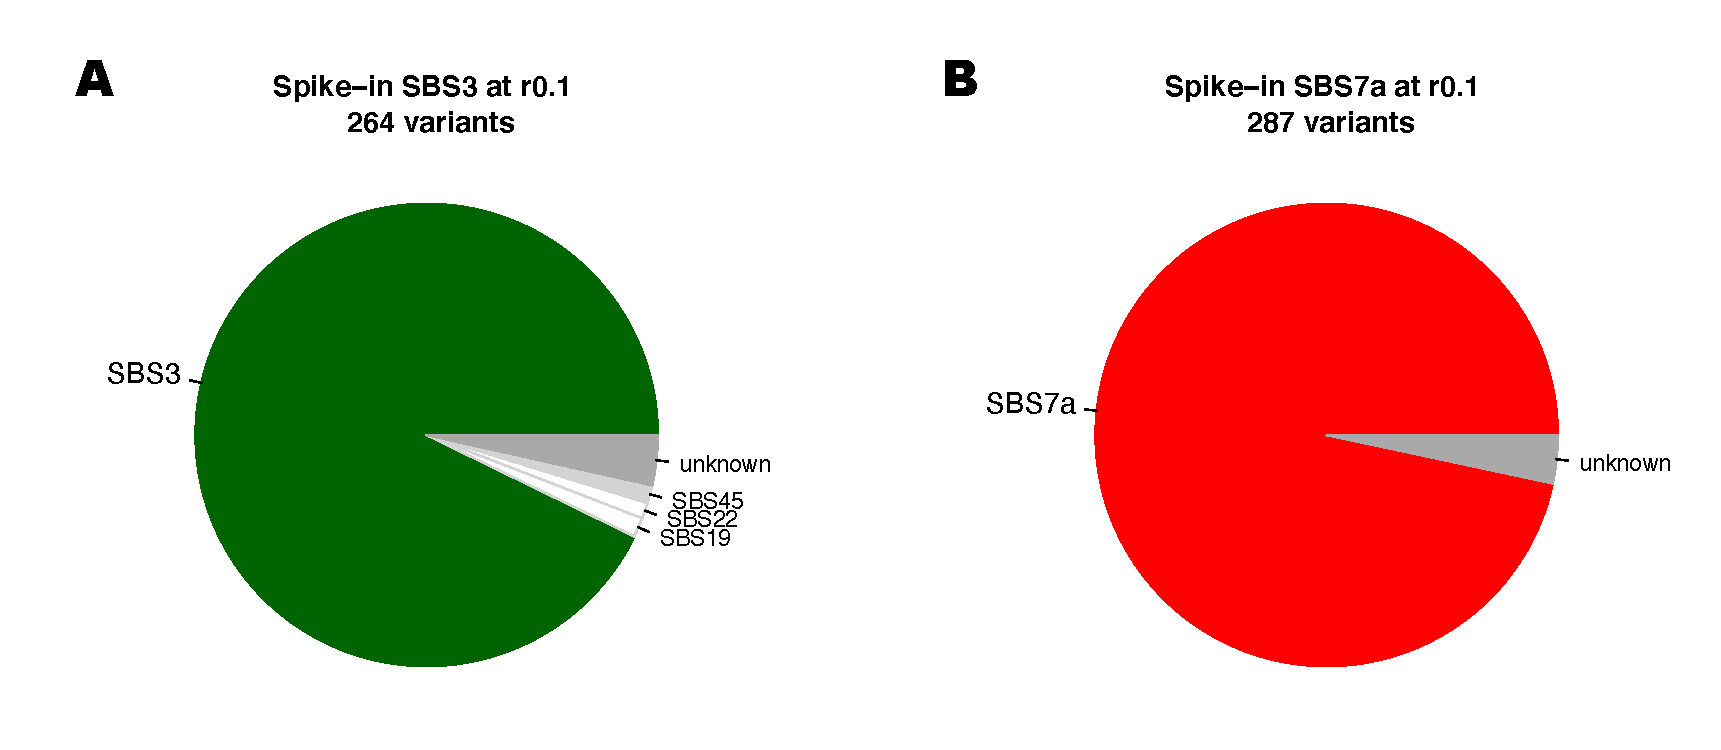
\includegraphics[width=.99\linewidth]{Figures/spikeInSanityCheck.pdf}
\caption[Signature analysis of spike-in somatic variants]{Signature analysis results of spiked-in somatic variants; signatures with a weight less than 1\% were collated into ``unknown``; The original spike-in signature was coloured in green (SBS3) and red (SBS7a), unrelated signatures are coloured white and signatures corresponding to sequencing artifacts are coloured in lightgrey; r0.1 corresponds to approximately 0.1 variants per mega base; Weights were generated with deconstructSigs \cite{Rosenthal2016} }\label{fig:mmf-spikeinsanity}
\end{figure}

The spike-in was done at multiple different ratios, to simulate varying tumour purity. \autoref{fig:mmf-spikeinsanity} shows the signature analysis result of the lowest spike-in ratio ``r0.1`` which corresponds to 0.1 somatic variants per mega base and results in approximately 300 variants for the whole genome. As the spike-in process has to satisfy certain quality measures, not all candidate variants can be used. As such, the final simulated BAM contains 264 additional variants for the SBS3 simulation and 287 for the SBS7a equivalent. That corresponds to 304 and 364 ``tumour`` reads respectively within the $\approx$ 261 million reads of the simulated BAM. With increasing ratio, the spike-in signatures show decreasing weights for other signatures, which likely got introduced due to the incomplete spike-in (\autoref{ch-mmfAppendix:spikein}).

\paragraph{Melanoma - UV exposure}
\label{mmf-sec:melaSim}

\todo[inline]{redo analysis with optimised (final) parameters}




\paragraph{BRCA1/2 - Defective homologous recombination-based DNA damage repair}
\label{mmf-sec:mbcSim}

\todo[inline]{redo analysis with optimised (final) parameters}

\subsubsection{Germline filtering}
\label{mmf-sec:germlinefiltering}
With real patient data, we can evaluate the effect of removing germline variants from the analysis is. For this I used the same simulated samples from above (\autoref{mmf-sec:simSingnatures}), where the reads are original ctDNA reads for a healthy person.

\subsubsection{Germline artifacts}
\label{mmf-sec:germlineArtifacts}
Now that we have shown how important the germline filtering step is to enable the method, we were interested, how many germline variants of the sample were still retained after our filtering with known variants (\autoref{mmf-sec:germline}). For this purpose I called germline variants on the original healthy individual using Strelka2 and compared the called variants with the sites which MisMatchFinder found to be somatic (retained after germline filtering)
\todo[inline,color=red]{do the analysis and make a figure}
\todo[inline,color=green]{discuss if this might be interesting to do for more healthies}





\subsection{Real world data - the only things that matters}
\label{mmf-sec:realworld}

\subsubsection{Healthy cohort}
\label{mmf-sec:healthy}

\todo[inline]{Add the health cohort in there/ possible age}

\subsubsection{BRCA positive patient samples}
\label{mmf-sec:brcapatients}
The first dataset of patients is two previously published BRCA1/2 positive breast cancers\todo{are they actually published?}. The data contains matched tumour, germline and ctDNA sequencing as high depth WGS for both patients. With the matched normal, we can use the current standard protocol of somatic mutational pattern analysis (\autoref{mmf-sec:signatureanalysis}) and compare it with our new method. 

As the sequencing data of the ctDNA is much higher depth than what is used in standard clinical practice, we down sample the data to 10x. By using numerous different seeds for the sampling, we can generate pseudo technical replicates of the sequencing (\autoref{ch-mmfAppendix:subsampling}), which then in term can give an approximation of the stability of the results for both the tissue and the ctDNA samples .

\todo[inline]{add the subsampled data}

\subsubsection{Melanoma patients}
\label{mmf-sec:melpatients}


\subsection{Summary}
\todo[inline]{Dont know if we need this}
